\documentclass{article}

\usepackage[portuguese]{babel}

\usepackage{amsmath, amssymb}
\usepackage{graphicx}
\usepackage[colorlinks=true, allcolors=blue]{hyperref}

\usepackage[section]{placeins}

\title{EFC 4}
\author{Vinícius de Oliveira Peixoto Rodrigues (245294)}
\date{Junho de 2022}

\begin{document}
\maketitle

\section*{Item (a)}

\begin{figure}[!ht]
    \centering
    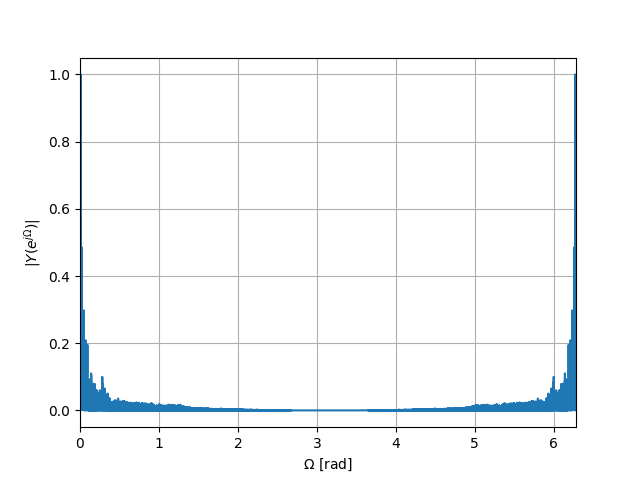
\includegraphics[width=\linewidth]{images/spectrum.png}
    \caption{Espectro de frequências do áudio \texttt{creed\_overcome.wav}}
\end{figure}

Observando a concentração de frequências próximas de $0$ (ou, equivalentemente, de $2\pi$), é possível afirmar que o áudio é formado majoritariamente por componentes de baixa frequência (como era de se esperar).

Apresentando uma estimativa um pouco mais quantitativa, a maior parte das frequências do espectro parecem estar concentradas abaixo de $\Omega = \pi/2$; convertendo para a frequência analógica equivalente:

\begin{gather*}
    T_s = 1/44100 \\
    \Omega = \omega T_s = 2\pi f T_s \Rightarrow f = \frac{\Omega}{2\pi T_s} =
        \frac{\pi/2}{2\pi \frac{1}{44100}} = \frac{44100}{4} = 11025 \text{ Hz}
\end{gather*}

Esse resultado faz sentido, visto que:

\begin{itemize}
    \item A maior parte das frequências da voz humana estão abaixo de 4 kHz (taxa de Nyquist: 8 kHz)
    \item A nota mais alta em uma guitarra (casa 24, em uma guitarra de 24 casas) tem aproximadamente 1318 Hz (taxa de Nyquist: 2.6 kHz)
    \item As frequências mais altas (particularmente do \textit{snare}) de uma bateria giram em torno de 5 kHz (taxa de Nyquist: 10 kHz)
\end{itemize}

Dessa forma, a maior parte das frequências relevantes dos instrumentos usados na gravação parecem estar dentro da região abaixo de 11 kHz no espectro do áudio.

\newpage
\section*{Item (b)}
\begin{figure}[!ht]
    \centering
    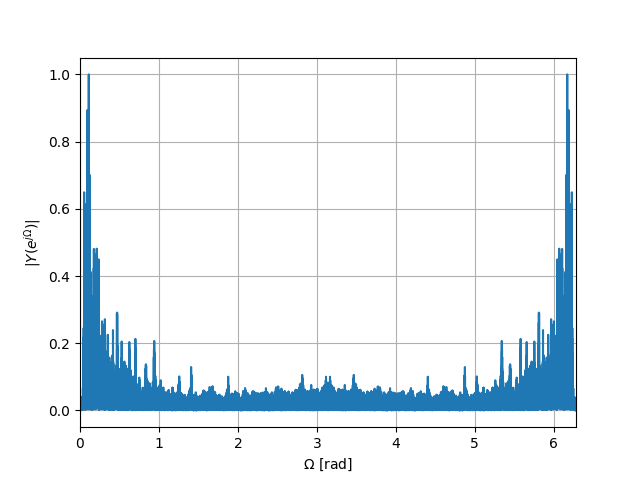
\includegraphics[width=\linewidth]{images/downsampled_spectrum.png}
    \caption{Espectro de frequências do sinal subamostrado}
\end{figure}

É possível ver claramente os efeitos do \textit{aliasing}, como o aumento das frequências mais altas e a distorção das mais baixas. Há também um aumento considerável dos "\textit{spikes}" no gráfico.

\section*{Item (c)}

Houve um aumento significativo do ruído no áudio; a introdução soa quase como se houvesse \textit{white noise} tocando de fundo, presumidamente devido ao aumento dos \text{spikes}/intensificação das altas frequências no espectro.

Também ficou significativamente mais difícil entender alguns trechos da letra da música, devido ao fato de que agora o áudio está com \textit{sample rate} de 4,4 kHz, significativamente abaixo da taxa de Nyquist calculada acima para a voz humana (8 kHz).

\newpage

\section*{Item (d)}
\FloatBarrier
\begin{figure}[!ht]
    \centering
    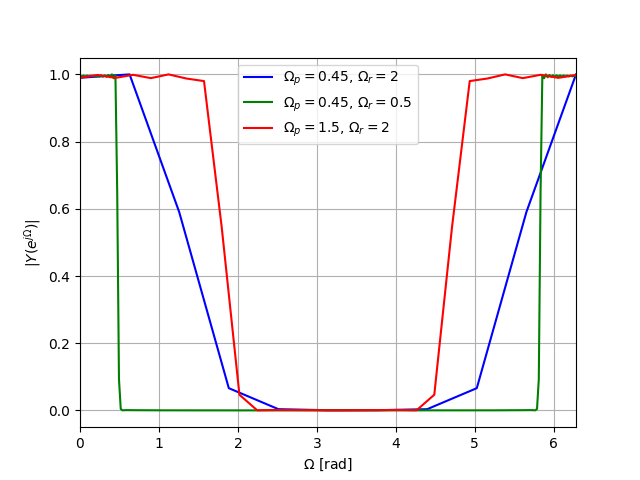
\includegraphics[width=\linewidth]{images/kaiser_freq_response.png}
    \caption{Resposta em frequência da janela de Kaiser}
\end{figure}

A resposta abaixo da frequência de passagem $\Omega_p$ é 1, e a resposta acima da frequência de $\Omega_r$ é 0.

\newpage
\section*{Item (e)}
\FloatBarrier
\begin{figure}[!ht]
    \centering
    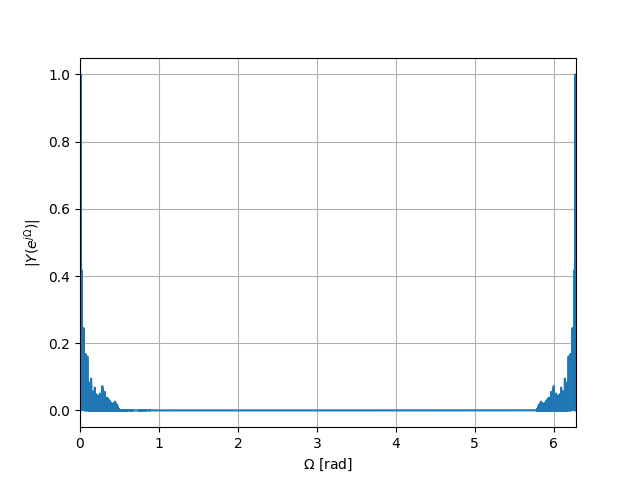
\includegraphics[width=\linewidth]{images/filtered_spectrum.png}
    \caption{Espectro do sinal filtrado com janela de Kaiser ($\Omega_p = 0.45$, $\Omega_r = 0.5$)}
\end{figure}

A qualidade do áudio caiu notavelmente, mas ainda é possível ouvir de forma relativamente clara o som dos instrumentos, e ainda é possível distinguir claramente as palavras da letra da música.
Isso faz sentido, visto que apesar de termos eliminado as frequências acima de $f = \frac{\Omega_r}{2\pi T_s} = \frac{0.5 \cdot 44100}{2\pi} = 3.5 \text{ kHz}$, boa parte das frequências da música (voz humana, guitarra, frequências mais baixas da bateria, etc) ainda estão abaixo desse limiar.

\newpage
\section*{Item (f)}
\FloatBarrier
\begin{figure}[!ht]
    \centering
    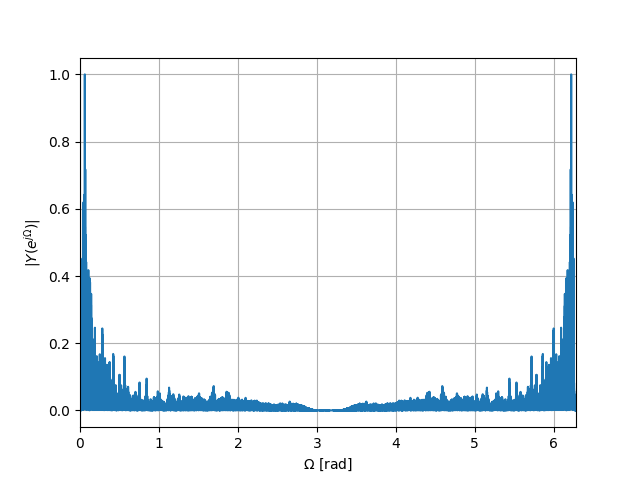
\includegraphics[width=\linewidth]{images/filtered_downsampled_spectrum.png}
    \caption{Espectro do sinal filtrado e \textit{downsampled} ($M=6$).}
\end{figure}

Apesar de a diferença entre os espectros ser visível (o sinal decimado tendo mais altas frequências que o filtrado do item anterior), a diferença sonora entre os dois é muito menos audível; há uma queda de qualidade na versão decimada que eu precisei me concentrar para perceber. A versão decimada parece possuir também um pouco mais de ruído (presumidamente devido ao aumento de intensidade das frequências mais altas).

\newpage
\section*{Item (g)}
\FloatBarrier
\begin{figure}[!ht]
    \centering
    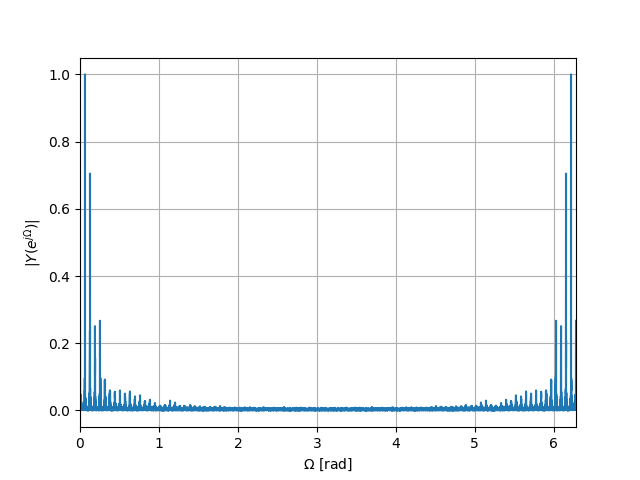
\includegraphics[width=\linewidth]{images/piano_note_spectrum.png}
    \caption{Espectro do áudio \texttt{piano\_note.wav}}
\end{figure}

A simetria nesse espectro (e em todos os outros espectros de sinais de áudio nesse relatório) se deve à propriedade da simetria conjugada da DFT; i.e.,

\begin{equation*}
    x[k] \in \mathbb{R} \Leftrightarrow X[k] = X^*[N-k]
\end{equation*}

visto que

\begin{gather*}
    X[k] = \sum_{n=0}^{N-1} x[k] e^{-j\frac{2\pi}{N}kn} \\
    \Rightarrow
    X[N-k] = \sum_{n=0}^{N-1} x[k] e^{-j\frac{2\pi}{N}(N-k)n} 
    = \sum_{n=0}^{N-1} x[k] \underbrace{e^{-j2\pi n}}_{=1} e^{-j\frac{2\pi}{N}(-nk)} \\
    = \sum_{n=0}^{N-1} x[k] e^{j\frac{2\pi}{N}nk}
    = \left(\sum_{n=0}^{N-1} x[k] e^{-j\frac{2\pi}{N}nk}\right)^*
    = X^*[k]
\end{gather*}

\section*{Item (h)}

A primeira ocorrência da máxima amplitude está em $k = 681$:

\begin{equation*}
    f = \frac{kf_s}{N} = \frac{681 \cdot 44100}{67936} = 442 \text{ Hz}
\end{equation*}

O que faz sentido, visto que a nota tocada no piano é um A4 (440 Hz na afinação padrão).

\section*{Item (g)}
\FloatBarrier
\begin{figure}[!ht]
    \centering
    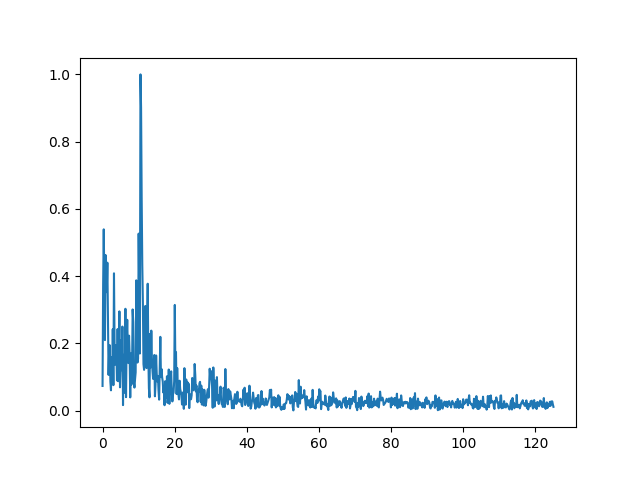
\includegraphics[width=\linewidth]{images/eeg_spectrum.png}
    \caption{Espectro do sinal do EEG.}
    \label{eeg_graph}
\end{figure}

O pico de frequência está visível no gráfico da Figura \ref{eeg_graph}, e corresponde à frequência analógica \boxed{10.5 \text{ Hz}}.

\end{document}
